\documentclass[lmodern, utf8, diplomski, numeric]{fer}
\usepackage{booktabs}

%\usepackage[activate={true,nocompatibility},final,tracking=true,kerning=true,spacing=true,factor=1500,stretch=10,shrink=10]{microtype}
\usepackage[final, stretch=25, shrink=15]{microtype}
\microtypecontext{spacing=nonfrench}
\usepackage{indentfirst}
\usepackage{booktabs}
\usepackage{tabularx}
\usepackage{caption}
\usepackage{rotating}

\usepackage[croatian]{babel}
\usepackage[utf8]{inputenc}
\usepackage[T1]{fontenc}

\usepackage{natbib}

\newcommand{\matr}[1]{\mathbold{#1}}
\newcommand{\graph}[1]{\mathcal{#1}}

\newcommand{\T}{\top}
\newcommand{\upto}{\mathinner {\ldotp \ldotp}}
\newcommand{\E}[1]{\operatorname{\mathbf{E}}\left[#1\right]}
\newcommand{\Var}[1]{\operatorname{\mathbf{Var}}\left[#1\right]}
\newcommand{\Efromto}[2]{\operatorname{\mathbf{E}}\left[#1\, \middle\vert\, #2\right]}
\newcommand{\Varfromto}[2]{\operatorname{\mathbf{Var}}\left[#1\, \middle\vert\, #2\right]}
\newcommand{\norm}[1]{\bar{#1}}
\newcommand{\prob}[1]{\operatorname{P}\left(#1\right)}
\newcommand{\R}[2]{\operatorname{\mathbf{R}}_{#1}\left[#2\right]}
\newcommand{\I}[1]{\operatorname{\mathrm{I}}\left(#1\right)}
\newcommand{\diff}{\operatorname{\mathrm{\Delta}}}
\newcommand{\diffn}[1]{\operatorname{\mathrm{\Delta}}^d}
\newcommand{\lag}{\operatorname{\mathrm{L}}}

\DeclareMathOperator*{\argmin}{arg\min}
\usepackage{fixmath}
\usepackage{array}
\usepackage{multirow}
\usepackage{bm}
\usepackage{mathrsfs}
\newcolumntype{C}{>{$}c<{$}}
\newcolumntype{R}{>{$}r<{$}}

\begin{document}

% TODO: Navedite broj rada.
\thesisnumber{1099}

% TODO: Navedite naslov rada.
\title{Analiza vremenskih nizova zasnovana na kompleksnim mrežama}

% TODO: Navedite vaše ime i prezime.
\author{Lovre Mrčela}

\maketitle

% Ispis stranice s napomenom o umetanju izvornika rada. Uklonite naredbu \izvornik ako želite izbaciti tu stranicu.
%\izvornik

% Dodavanje zahvale ili prazne stranice. Ako ne želite dodati zahvalu, naredbu ostavite radi prazne stranice.
\zahvala{Zahvaljujem se dopredsjednici Hrvatskog sabora dr. sc. Vesni-Ani Škaro i Miloradu Pupovcu.}

\tableofcontents

\chapter{Uvod}
%  Classical statistical arbitrage methods take into account a pair of assets whose prices behave similarly during certain period of time.
%  Similarity is measured by cointegration, correlation, or some other measure in order to find a moment in time when those assets' prices exceed what was statistically determined as highly confident range.
%  When such opportunities present themselves, we can take advantage by predicting that prices will return once again to the confident range in the next time step, and do the trading in accordance with this prediction.
  Klasične metode statističke arbitraže uzimaju u obzir parove vrijednosnica čije cijene se ponašaju slično tijekom određenom vremenskog perioda.
  Sličnost se mjeri kointegracijom, korelacijom, ili nekom drugom mjerom, s ciljem pronalaska trenutka kada te cijene izlaze van statistički utvrđenog intervala visoke pouzdanosti.
  Takve prilike mogu se iskoristiti predviđanjem da će se cijene u idućem trenutku ponovno vratiti unutar intervala visoke pouzdanosti, te se u skladu s tim predviđanjem može provesti trgovanje.
  
%  In this paper, we propose a new method based on those predictions that are obtained by the statistical arbitrage method, using statistical measures as a proxy for describing the preference relations between pairs of assets.
%  Next, a graph is formed based on those relations, so that mutual interaction of assets might be analyzed.
%  This graph imposes a preference relation among the assets that are included in it.
%  Finally, assets are sorted by preference and included into the portfolio.
%  The idea of this method is to create a generalization of statistical arbitrage methods that is more robust and performs better when working with a larger number of assets by trying to take into account mutual interaction of assets.

  U ovom radu, predložena je nova metoda temeljena na predviđanjima koja su dobivena metodom statističke arbitraže, pri čemu se statističke mjere koriste za opisivanje relacije preferencije među parovima vrijednosnica.
  Razlikuju se dvije vrste preferencije: preferencija jedne vrijednosnice nad drugom i individualna mjera preferencije za svaku vrijednosnicu.
  Iz dobivene relacije preferencije konstruira se graf toka preferencija iz kojeg se može proučiti međusobna interakcija svih vrijednosnica koje su na raspolaganju.
%  Idući korak je konstruiranje grafova temeljenih na prethodno dobivenim relacijama, kako bi se mogla proučiti međusobna interakcija svih vrijednosnica koje su na raspolaganju.
  Konačno, za svaku vrijednosnicu izračunava se individualna mjera preferencije, na temelju čega se donosi odluka o sastavljanju portfelja.
  
  Ideja ove metode je ostvariti generalizaciju klasičnih metoda statističke arbitraže koja će biti robusnija i ostvarivati bolje rezultate kada ima velik broj vrijednosnica na raspolaganju tako što izvlači zajedničku interakciju iz svih vrijednosnica.

\chapter{Metode i koncepti}
  Ovdje su opisane matematičke metode i koncepti koji su korišteni u radu.
  Ako vam se ne sviđa slobodno možete preskočit...

  \section{Statistička arbitraža}
  Statistička arbitraža \engl{statistical arbitrage} je algoritam trgovanja zasnovan na statistici.
  Pojam arbitraža u kontekstu financija označava okolnosti pod kojima se može konstruirati portfelj koji ostvaruje pozitivan profit s vjerojatnošću 1, dok pritom njegova početna vrijednost iznosi 0.
  Trivijalan primjer arbitraže je situacija u kojoj bi se ista vrijednosnica nudila po različitoj cijeni na dva različita tržišta, i tada je arbitražu moguće ostvariti kupovanjem vrijednosnice po nižoj cijeni na jednom tržištu i prodavanjem po višoj na drugom.
  Matematička definicija arbitražnih okolnosti je sljedeća:
  \begin{equation}
  \label{eq:statarb}
  V^{(0)} = 0, \quad \prob{V^{\left(t\right)} > 0} = 1,
  \end{equation}
  gdje $V^{\left(t\right)}$ označava vrijednost portfelja u trenutku $t$.

  U statističkoj arbitraži cilj je eksploatirati statističke zakonitosti koje vrijede među parovima vrijednosnica kako bi se ostvario profit.  
  Valja napomenuti da, iako nosi naziv arbitraža, statistička arbitraža zapravo ne zadovoljava nužno (\ref{eq:statarb}), jer korištene statističke mjere imaju određeni interval pouzdanosti koji je manji od 1.
  Tako se može može dogoditi da bude $V^{\left(t\right)} < 0$ za neke $t$.
  Ipak, kako $t \to +\infty$, vjerojatnost $\prob{V^{\left(t\right)} > 0} \to 1$.
  U praksi, potrebno je osigurati dovoljno velik početni iznos $V^{(0)}$ kako bi se izbjegla mogućnost \textit{defaulta}.
  
  Algoritam statističke arbitraže najčešće čine sljedeći koraci (za svaki vremenski trenutak):
  \begin{enumerate}
    \item određivanje neke mjere sličnosti među parovima vrijednosnica nad proteklim vremenskim periodom zadane duljine,
    \item uzimanje u obzir samo onih parova kod kojih mjera sličnosti ne prelazi zadani prag, odnosno odbacivanje preostalih parova;
    \item za parove čije je ponašanje međusobno dovoljno slično utvrđuje se nalaze li se u sadašnjem trenutku njihove cijene izvan očekivanog intervala,
    \item u skladu s utvrđenim provodi se trgovanje parovima vrijednosnica na način da se u jednoj od njih zauzme kratka, a u drugoj duga pozicija, te se u idućem trenutku te pozicije resetiraju.
  \end{enumerate}
  
  Najčešće korištene mjere sličnosti su: razlika normaliziranih log-cijena, normalizirana razlika log-cijena, te kointegracija slučajnih procesa.
  U nastavku su ukratko opisane navedene mjere.
  
  \subsection{Razlika normaliziranih log-cijena}
  Neka je sa $P_X^{\left(t\right)}$ označena log-cijena vrijednosnice $X$ u trenutku $t$, i neka se koristi period od $T$ vremenskih koraka.
  Neka je ukupno $M$ vremenskih koraka, tj. $t \in \left[0, 1, \ldots, M - 1\right]$.
  Za svaku vrijednosnicu $X$ u trenutcima $t \ge T$ izračunaju se normalizirane log-cijene $\norm{P}_X^{\left(t\right)}$:
  \begin{equation}
  \norm{P}_X^{\left(t\right)} = \frac{P_X^{\left(t\right)} - \Efromto{P_X^{(\tau)}}{t-T \le \tau < t}}{\sqrt{\Varfromto{P_X^{(\tau)}}{t-T \le \tau < t}}}.
  \end{equation}
  Oznake $\Efromto{P_X^{(\tau)}}{t_1 \le \tau < t_2}$ i $\Varfromto{P_X^{(\tau)}}{t_1 \le \tau < t_2}$ predstavljaju očekivanje i varijancu cijene vrijednosnice $X$ nad intervalom $\left[t_1, t_2\right>$.
  Nadalje, za svaki par vrijednosnica $X$ i $Y$ izračuna se razlika njihovih normaliziranih log-cijena $D_{X,Y}^{\left(t\right)}$ u trenutku $t$:
  \begin{equation}
  D_{X,Y}^{\left(t\right)} = \norm{P}_X^{\left(t\right)} - \norm{P}_Y^{\left(t\right)}
  \end{equation}
  Razlika normaliziranih log-cijena se koristi kao mjera sličnosti u algoritmu statističke arbitraže.
  Kod ove mjere normalizacijom se postiže ravnopravna usporedba dviju dionica različitih volatilnosti, što znači da će se prilikom usporedbe dviju dionica čiji su intenziteti promjene cijene različiti nakon normalizacije oni dovesti na istu razinu.
  
  \subsection{Normalizirana razlika log-cijena}
  Za razliku od prethodne mjere sličnosti, u ovom slučaju se razlika računa nad nenormaliziranim log-cijenama za sve $t$, označeno sa $d_{X,Y}^{\left(t\right)}$:
  \begin{equation}
  d_{X,Y}^{\left(t\right)} = P_X^{\left(t\right)} - P_Y^{\left(t\right)},
  \end{equation}
  a zatim se iz razlika $d_{X,Y}^{\left(t\right)}$ računaju normalizirane razlike $\norm{d}_{X,Y}^{\left(t\right)}$ za $t \ge T$:
  \begin{equation}
  \norm{d}_{X,Y}^{\left(t\right)} = \frac{d_{X,Y}^{\left(t\right)} - \Efromto{d_{X,Y}^{(\tau)}}{t-T \le \tau < t}}{\sqrt{\Varfromto{d_{X,Y}^{(\tau)}}{t-T \le \tau < t}}}.
  \end{equation}
  Ovako dobivena normalizirana razlika log-cijena koristi se kao mjera sličnosti.
  U odnosu na prethodnu, ova mjera je više osjetljiva na promjene log-cijena neovisno o volatilnostima samih vrijednosnica, što će doći do izražaja prilikom usporedbe dviju vrijednosnica čije se cijene mijenjaju različitom brzinom i intenzitetom.
  
  \subsection{Mjera kointegracije za slučajne procese}
  Za razliku od prethodne dvije mjere sličnosti gdje se cijene dionica tretiraju kao vremenski nizovi, kod ove mjere one se tretiraju kao realizacije slučajnog procesa.
  Za neki slučajni proces zanimljivo je proučiti svojstvo stacionarnosti --- slučajni proces $U\left[t\right]$ je stacionaran ako i samo ako vrijedi:
  \begin{gather}
  \label{eq:stat1}
  \E{U\left[t\right]} = \mathrm{const.}\\
  \label{eq:stat2}
  \R{UU}{t, \tau} = \E{U\left[t\right] \cdot U\left[t + \tau\right]} = \R{UU}{\tau}.
  \end{gather}
  Za stacionarne slučajne procese vrijedi da njihova statistička svojstva ne ovise o vremenu:
  jednadžba (\ref{eq:stat1}) tvrdi da je za stacionaran proces $U\left[t\right]$ srednja vrijednost slučajnog procesa $\E{U\left[t\right]}$ neovisna o vremenu $t$, a jednadžba (\ref{eq:stat2}) tvrdi da njegova autokorelacija $\R{UU}{t, \tau}$ ovisi samo o vremenskom pomaku $\tau$, ali ne i o $t$.
  Ovakva definicija stacionarnosti naziva se još i ``stacionarnost u širem smislu''.
  
  Red integracije slučajnog procesa, označen sa $\I{d}$, gdje je $d$ red integracije, opisuje njegovu stacionarnost.
  Stacionarni slučajni procesi su $\I{0}$.
  Za općenit proces $V\left[t\right]$ koji je $\I{1}$ vrijedi da je proces $\diff V\left[t\right]$ dobiven njegovim diferenciranjem
  \begin{equation}
  \label{eq:red1}
  \diff V\left[t\right] = \left(1 - \lag\right) V\left[t\right] = V\left[t\right] - V\left[t - 1\right]
  \end{equation}
  stacionaran proces, a za općenit proces $W\left[t\right]$ koji je $\I{d}$ vrijedi da je proces $\diffn{d} W\left[d\right]$ dobiven njegovim uzastopnim diferenciranjem $d$ puta
  \begin{align}
  \diffn{d} W\left[t\right] &= \left(1 - \lag\right)^d W\left[t\right] = \left( \sum_{n = 0}^{d} \binom{d}{n} \left(-1\right)^n\lag^n \right) W\left[t\right] \nonumber \\
  \label{eq:redn}
  &= \sum_{n = 0}^{d} \binom{d}{n} \left(-1\right)^n W\left[t - n\right]
  \end{align}
  stacionaran proces.
  U (\ref{eq:red1}) i (\ref{eq:redn}) korišten je operator kašnjenja $\lag$ sa značenjem $\lag U\left[t\right] = U\left[t - 1\right]$.
  
  Trivijalno je provjeriti da linearna kombinacija dvaju slučajnih procesa koji su $\I{0}$ jest također $\I{0}$, kao i da linearna kombinacija dvaju slučajnih procesa od kojih je jedan $\I{0}$, a drugi $\I{1}$ jest $\I{1}$.
  Malo je teže odrediti kojeg je reda integracije linearna kombinacija dvaju slučajnih procesa koji su $\I{1}$: to može biti $\I{0}$ ili $\I{1}$.
  Kointegracija dvaju slučajnih procesa $X\left[t\right]$ i $Y\left[t\right]$ koji su $\I{1}$ označava da je njihova linearna kombinacija $U\left[t\right]$ stacionaran proces, odnosno $\I{0}$:
  \begin{equation}
  X\left[t\right] + \beta Y\left[t\right] = U\left[t\right],
  \end{equation}
  gdje je $\beta$ konstanta koja se još naziva i kointegracijski koeficijent.
  Stacionarni slučajni proces $U\left[t\right]$ pritom se može prikazati kao:
  \begin{equation}
  U\left[t\right] = \mu + \varepsilon\left[t\right],
  \end{equation}
  gdje je $\mu = \E{U\left[t\right]}$, srednja vrijednost, a $\varepsilon\left[t\right]$ rezidualna vrijednost za koju vrijedi $\E{\varepsilon\left[t\right]} = 0$.
  
  Pretpostavka kod ove mjere sličnosti jest da su dva nestacionarna slučajna procesa $P_X\left[t\right]$ i $P_Y\left[t\right]$ koji predstavljaju kretanje log-cijena vrijednosnica $X$ i $Y$ kointegirana.
  Postoji nekoliko metoda za provjeru kointegracije, najčešće korištene su Engle-Granger metoda, Johansen metoda i Phillips-Ouliaris metoda.
  Najjednostavnija od navedenih je Engle-Granger metoda, koja je opisana u nastavku.
  
  Ideja metode Engle-Granger je u prvom koraku estimirati stacionaran proces $U\left[t\right]$ koji je linearna kombinacija cijena $P_X\left[t\right]$ i $P_Y\left[t\right]$, zatim u drugom koraku provjeriti\ldots
  Postupkom najmanjih kvadrata najprije se određuju procjene parametara $\mu$ i $\beta$, označene sa $\hat{\mu}$ i $\hat{\beta}$:
  \begin{equation}
  \hat{\mu}, \hat{\beta} = \argmin_{\mu, \beta} \left\{\left\lVert P_X\left[t\right] + \beta P_Y\left[t\right] -\mu \right\rVert^2\right\},
  \end{equation}
  a zatim se izraze procijenjene rezidualne vrijednosti $\hat{\varepsilon}\left[t\right]$:
  \begin{equation}
  \hat{\varepsilon}\left[t\right] = -\hat{\mu} + P_X\left[t\right] + \hat{\beta} P_Y\left[t\right].
  \end{equation}
  
  
  Testovi kointegracije, koji postoje.
  
  Koja je mjera sličnosti?
  
  Nedostatak: zahtjevni izračuni, pogotovo za velik broj parova.
  
  \subsection{Nedostaci statističke arbitraže}
  
  Nedostaci klasičnih metoda statističke arbitraže su: faljivanje. Kad se uključe troškovi trgovanja...

  \section{Relacija preferencije i funkcija korisnosti}

%  Let $\Omega$ be any set of entities.
  Neka je $\Omega$ skup općenitih dobara.
%  Preference relation $\succ$ defined over $\Omega \times \Omega$ is a strict weak ordering that describes the way humans prefer some entity over another.
  Relacija preferencije, označena sa $\succ$ i definirana nad $\Omega \times \Omega$, je strogi slabi uređaj koji odgovara načinu na koji ljudi preferiraju jednu vrijednosnicu u odnosu na drugu.
  Između dvaju dobara $a, b \in \Omega$ relacija može, ali i ne mora postojati.
  Primjerice, $a$ može biti više preferirano u odnosu na $b$, ili $b$ u odnosu na $a$, ali moguća je situacija gdje su oba dobra podjednako preferirana.
  U tom slučaju radi se o indiferentnosti između $a$ i $b$, i to se označava kao $a \sim b$.
%  This relation is specific in that it is ($\forall x, y, z \in \Omega$):

  Ova relacija specifična je po tome što je:
  \begin{itemize}
%    \item \textit{irreflexive}: every entity $x$ is not preferrable over itself, %($\neg \left( x \succ x \right)$),
    \item \textit{irrefleksivna}: $\forall x \in \Omega\colon \neg \left( x \succ x \right)$ --- za nijedno dobro ne vrijedi da je više preferirano od samog sebe,
%    \item \textit{asymmetrical}: if $x$ is preferrable over some $y$, then $y$ is not preferrable over $x$, %($x \succ y \Rightarrow \neg \left( y \succ x \right)$),
    \item \textit{asimetrična}: $\forall x, y \in \Omega\colon x \succ y \Rightarrow \neg \left( y \succ x \right)$ --- ako je $x$ više preferirano od $y$, onda $y$ nije više preferirano od $x$,
%    \item \textit{transitive}: if $x$ is preferrable over $y$, and $y$ is preferrable over $z$, then $x$ is also preferrable over $z$, %($x \succ y \wedge y \succ z \Rightarrow x \succ z$),
    \item \textit{tranzitivna}: $\forall x, y, z \in \Omega\colon x \succ y \wedge y \succ z \Rightarrow x \succ z$ --- ako je $x$ više preferirano od $y$, te $y$ više preferirano od $z$, tada je i $x$ više preferirano od $z$,
%    \item \textit{transitive in incomparability} (noting that $x$ and $y$ may be \textit{incomparable}, i.e. neither $x$ is preferrable over $y$, nor $y$ is preferrable over $x$): if $x$ is incomparable with $y$, and $y$ is incomparable with $z$, then $x$ is also incomparable with $z$.
    \item \textit{tranzitivna po indiferentnosti}: $\forall x, y, z \in \Omega\colon x \sim y \wedge y \sim z \Rightarrow x \sim z$ --- ako je $x$ podjednako preferirano kao i $y$, te $y$ podjednako preferirano kao i $z$, tada je i $x$ podjednako preferirano kao i $z$.
  \end{itemize}
  
%  We naturally assume this kind of relation we describe relationships among the assets.
%  Determining that some asset is preferred over another is easier than assigning a preference rank to each asset individually, especially for a larger number of assets.
%  However, the latter is more useful for decision making, and therefore it is desirable to find a way of sorting assets in the order of preference.
  Ovakva vrsta relacije prirodno opisuje odnose među različitim vrijednosnicama, npr. dionica $A$ u nekom trenutku može biti više preferirana od dionice $B$.
  Razlog tome je što je za čovjeka lakše ocijeniti odnos (više, manje, jednako preferirano) između svakog para vrijednosnica, nego pridijeliti svakoj vrijednosnici individualnu mjeru preferencije, pogotovo ako se radi o velikom broju vrijednosnica.
  No ipak, u svrhu konstruiranja portfelja korisnije je posjedovati individualnu mjeru preferencije za svaku vrijednosnicu.
  Stoga je poželjno pronaći način da se iz relacije preferencije dobiju individualne mjere preferencije.
  
%  Utility function $U\colon \Omega \to \mathbb{R}$ is mapping from entities to real numbers, in such way that order of the mapping corresponds to the preference order of the entities, i.e. $\forall x, y \in \Omega, U(x) > U(y) \Rightarrow x \succ y$.
%  One such mapping is obtained by using potential method that is described later in this paper.
%  In addition to ordering of the entities, utility function also provides the intensity of preference for a particular entity, hence it is more informative when it comes to the decision making.
  Funkcija korisnosti \engl{utility function} $U\colon \Omega \to \mathbb{R}$ je preslikavanje iz skupa dobara u skup realnih brojeva, na način da poredak preslikanih realnih brojeva odgovara poretku dobara prema individualnoj preferenciji, tj. vrijedi $\forall x, y \in \Omega \colon U(x) > U(y) \Leftrightarrow x \succ y$.
  Jedno takvo preslikavanje ostvaruje se korištenjem metode potencijala koja je opisana u poglavlju \ref{sec:metpot}.
  Uz to što određuje poredak dobara prema individualnoj preferenciji, funkcija korisnosti također unosi i mjeru intenziteta preferencije prema nekoj vrijednosnici, što znači da nosi više informacija od same relacije.

  \section{Graf toka preferencija}
  
%  Graph of preference flow is a weighted directed graph without multiple edges and loops, whose nodes represent entities, edges represent preference for one entity over another, and edge weights correspond to the strength of the preferences.
%  If an edge between nodes is missing, it is considered that neither entity is preferable over another (incomparability of entities).
%  The graph as a whole describes preference flow among the entities.
%  An example of graph is shown on Fig. \ref{fig:graph}.
  Graf toka preferencija je težinski usmjereni graf, bez višestrukih bridova i petlji.
  Njegovi čvorovi predstavljaju vrijednosnice, usmjereni bridovi preferenciju jedne vrijednosnice nad drugom, a težine bridova odgovaraju intenzitetu preferencije.
  Ukoliko između dva čvora nedostaje brid, smatra se da su pripadne vrijednosnice podjednako preferirane (indiferentnost u odlučivanju).
  Graf kao cjelina opisuje tok preferencija među vrijednosnicama.
  Primjer grafa prikazan je na slici \ref{fig:graph}.
  
  \begin{figure}[h]
    \centering
    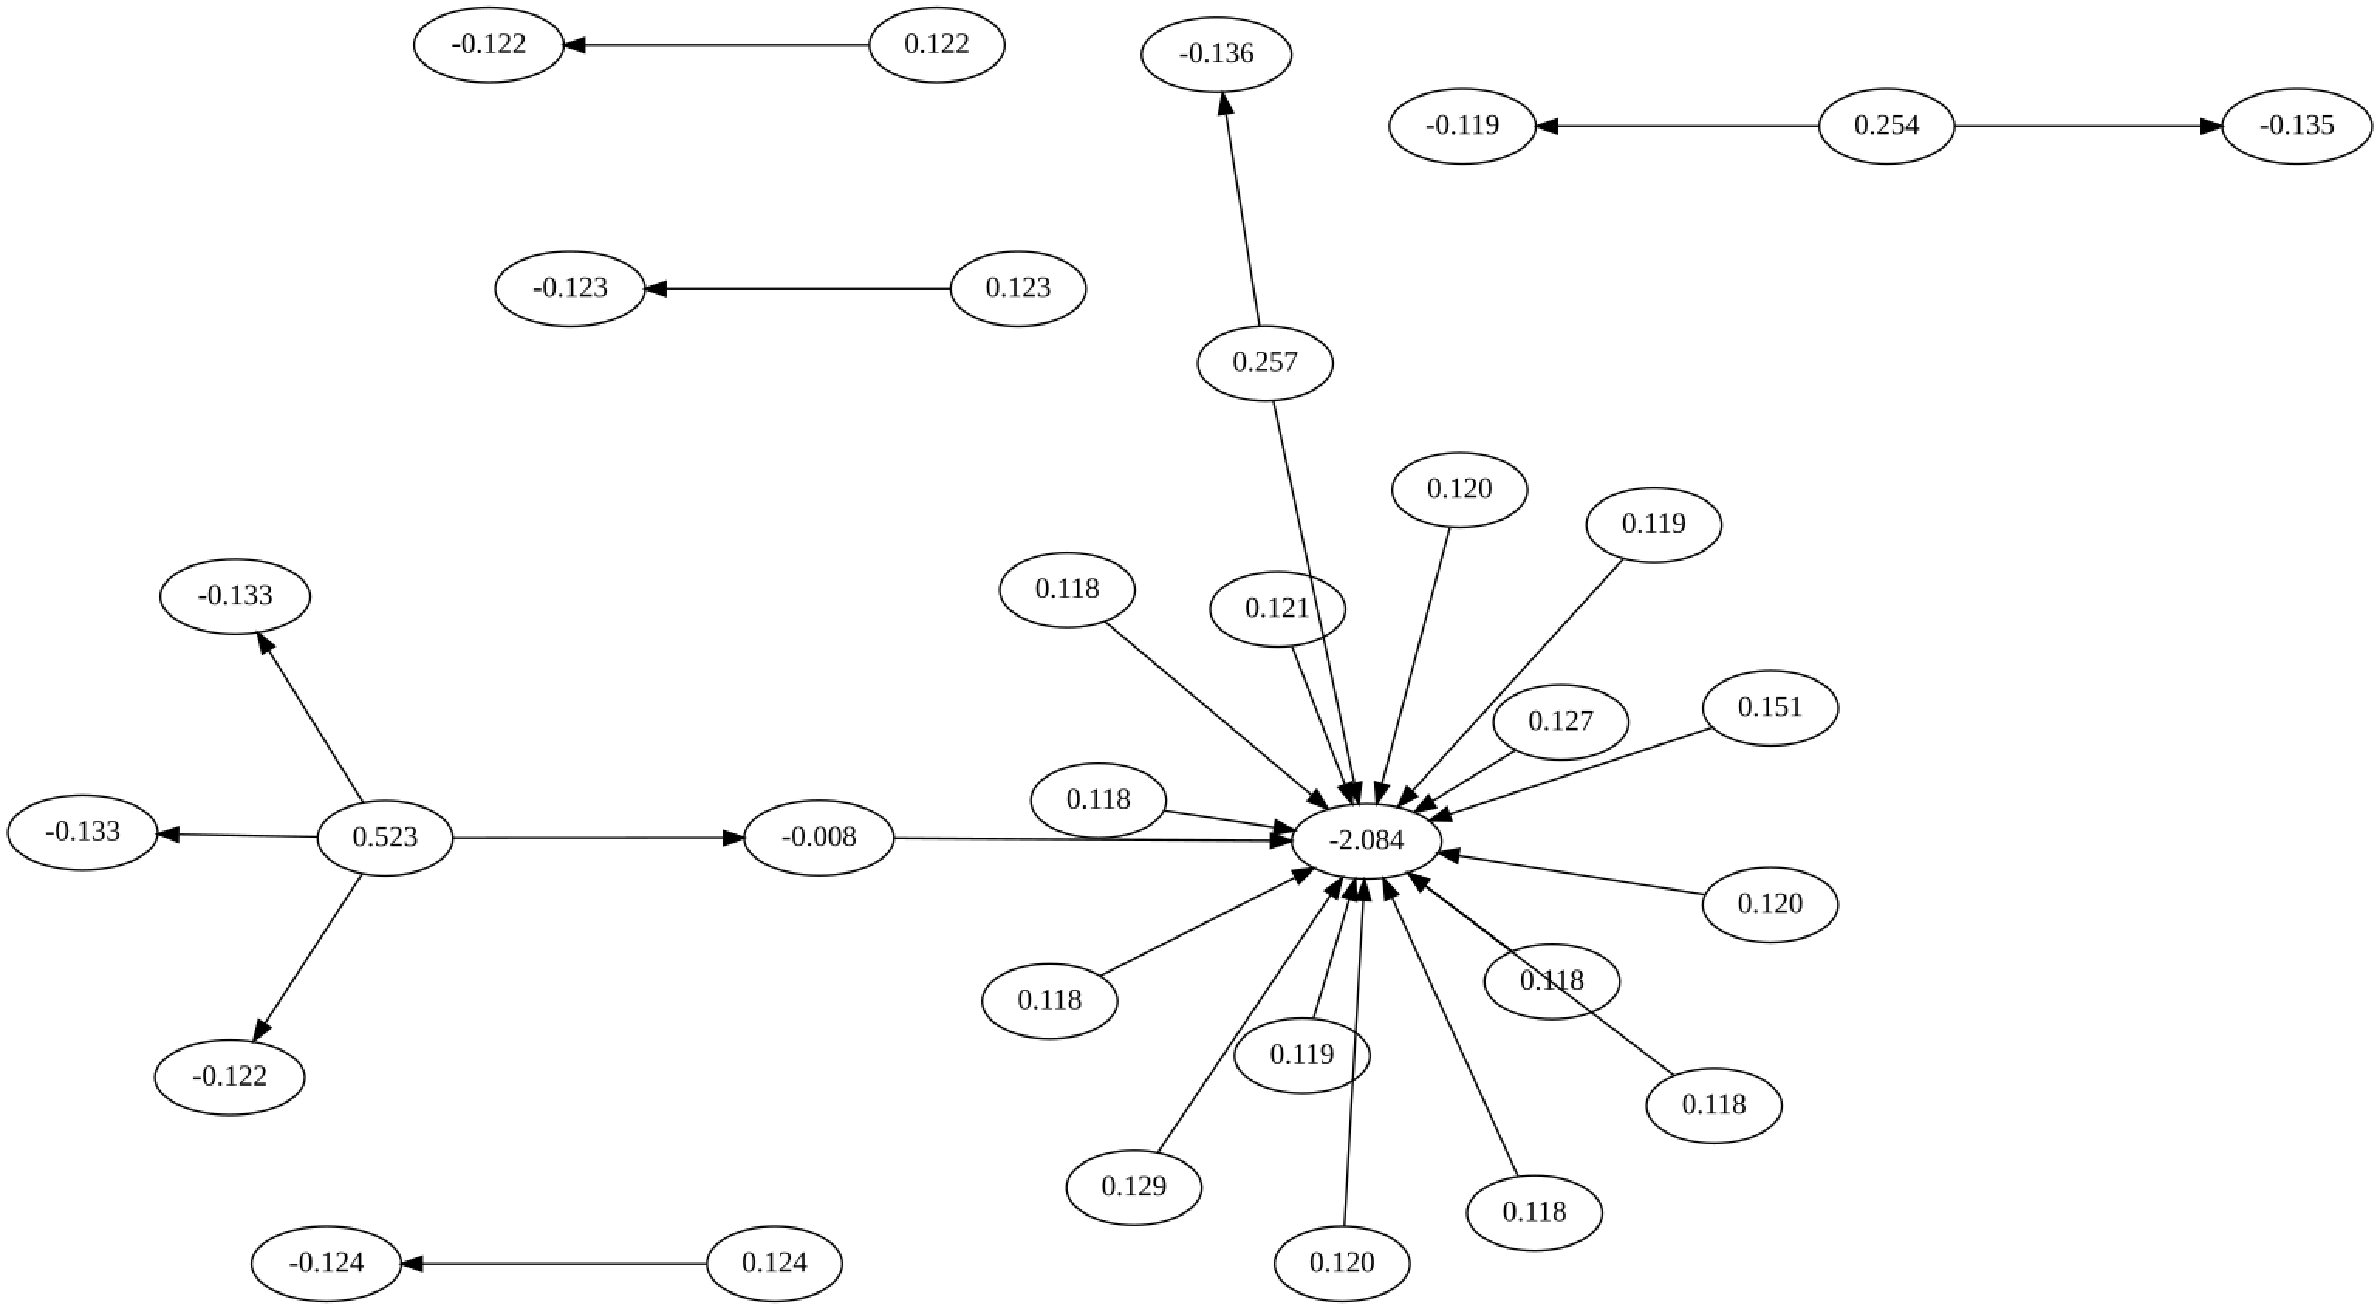
\includegraphics[width=0.6\columnwidth]{graphics/graph.pdf}
    \caption{Primjer grafa toka preferencija. Na bridovima su prikazani intenziteti preferencija jedne vrijednosnice u odnosu na drugu, a u čvorove su upisane izračunate individualne mjere preferencija za pripadnu vrijednosnicu.}
    \label{fig:graph}
  \end{figure}
  
%  Construction of the graph is based on a statistical arbitrage method.
%  An edge going from node $i$ to node $j$ with weight $w_{i,j}$ will be present in the graph if and only if assets represented by nodes $i$ and $j$ have demonstrated similar behavior during the past period, but have suddenly diverged at the moment, as determined per statistical measures.
%  Weight $w_{i,j}$ corresponds to the magnitude of this divergence.  
%  A detailed description of used statistical measures the procedure is given later in \ref{sub:creating-graph}.
  Konstrukcija grafa temelji se na metodi statističke arbitraže.
  Brid koji ide od čvora $i$ do čvora $j$ s težinom $w_{i,j}$ je prisutan u grafu ako i samo ako su se dvije pripadne vrijednosnice $i$ i $j$ ponašale slično tijekom proteklog vremenskog perioda, ali su prema određenim statističkim mjerama trenutačno razdvojile.
  Težina $w_{i,j}$ opisuje magnitudu ovog razdvajanja.
  Detaljan opis korištenih statističkih mjera dan je u odjeljku \ref{sub:creating-graph}.
    
%  Connections in this graph impose a preference relation among entities that are presented by the graph, in the way that an edge that goes from node $A$ to node $B$ means that $A$ is preferred over $B$.
%  It is the case that neither node is in relation with itself (irreflexivity), and that no multiple connections are allowed between two nodes (implies asymmetry).
%  However, problems arise with the aforementioned properties of transitivity, and transitivity in incomparability, which may not hold for an arbitrarily constructed instance of the graph.
%  This imposed preference relation should preferably be in compliance with all the aforementioned properties, but when it comes to larger number of entities, it may become infeasible to construct a graph of such qualities directly.
%  Instead of aiming at a consistent preference relation, we devise a consistency measure that describes similarity between the original graph and its nearest consistent reconstruction, and use it as an additional parameter in decision making.
  Veze u ovom grafu nameću relaciju preferencije među vrijednosnicama koje su opisane grafom, na način da brid koji ide iz čvora $i$ u čvor $j$ pokazuje da je vrijednosnica $i$ više preferirana od vrijednosnice $j$.
  Kako ne graf sadrži petlje, tj. nijedna vrijednosnica nije u relaciji sama sa sobom, ispunjeno je svojstvo irrefleksivnosti; a kako nema višestrukih bridova među čvorovima vrijedi i svojstvo asimetričnosti.
  Ipak, problemi se pojavljuju kod prethodno spomenutih svojstava tranzitivnosti, i tranzitivnosti po indiferentnosti, koja ne moraju uvijek vrijediti za proizvoljno konstruiran graf.
  Poželjno bi bilo da relacija preferencije koju graf nameće zadovoljava sva četiri prethodno navedena svojstva; no konstruiranje grafa koji posjeduje takva svojstva je nepraktično, pogotovo kada se radi o većem broju vrijednosnica.
  
  Umjesto da cilj bude konstrukcija grafa koji će biti konzistentan sa svojstvima relacije preferencije, definirana je mjera konzistentnosti koja opisuje koliko je neki graf sličan sa svojom najbližom konzistentnom rekonstrukcijom.
  Mjera konzistentnosti se koristi kao dodatan parametar pri konstruiranju portfelja.
  Opis mjere konzistentnosti te način dobivanja najbliže konzistentne rekonstrukcije grafa dan je u odjeljku \ref{sec:metpot}.
  
  %  The measure of this preference flow is determined by a statistical arbitrage method, and it corresponds to the magnitude of a pair of assets prices ratio going out of what is considered statistically confident range.
  %  
  
  %Preference of a node itself corresponds to the difference between the amount of flow going in and out of it.
  
  %  The main idea of preference flow is that preference for a particular node depends on amount of preference which flows in and out of it.
  %  This allows for some kind of generalized statistical arbitrage over multiple assets at a time.

  \section{Metoda potencijala}
  \label{sec:metpot}
%  From previously obtained graph it is possible to tell which pair of assets has the highest preference flow.
%  However, it is not yet possible to directly tell which are the most or least preferrable assets, or obtain the measure of preference for individual assets.
%  To calculate preferences for each node in the graph, we use the potential method\cite{caklovic}.
%  The potential of a node corresponds to difference in amount of flow going in and out of the node.
  Iz prethodno dobivenog grafa moguće je utvrditi u kojem paru vrijednosnica je tok preferencije najveći.
  Ipak, još uvijek nije moguće izravno utvrditi koja konkretna vrijednosnica je najviše ili najmanje poželjna, ili odrediti individualne mjere preferencije za svaku vrijednosnicu.
  Kako bi to bilo moguće korištena je metoda potencijala koja je opisana u nastavku.
  
  %  A concise summary of the method is as follows:
  %  \begin{enumerate}
  %    \item 
%  For the observed graph $\graph{G}$, let there be a total of $N$ nodes, and maximum of $E = \binom{N}{2}$ edges, in case of a complete graph.
%  If $\graph{G}$ is not complete, we complete it by adding edges to it with weight 0 (direction doesn't matter),
%  thus forming a complete graph $\graph{G}$ with $\binom{N}{2}$ edges.
  % In our case, graphs will be incomplete for most of the time, but they may be \textsl{supplemented} (TODO: opposite of `reduced') to complete graphs, if we treat missing edges as edges of weight 0 (direction doesn't matter).
  
  \subsection{Računanje potencijala čvorova}
  \label{sub:potential}
  Neka je za promatrani graf $\graph{G}$ ukupno $N$ čvorova, te najviše $E = \binom{N}{2}$ bridova, ukoliko se radi o potpunom grafu.
  Ako $\graph{G}$ nije potpun graf, on se može dopuniti na način da se dodaju bridovi između čvorova koji nisu povezani, čija je težina jednaka 0, a sam smjer nije bitan.
  U nastavku se podrazumijeva da je $\graph{G}$ potpun graf.
  
  %    \item
%  Let $\matr{B}$ be the $E \times N$ incidence matrix of $\graph{G}$.
  Neka je $\matr{B}$ matrica incidencije grafa $\graph{G}$.
  Matrica incidencije je matrica za koju vrijedi:
  \begin{enumerate}
    \item broj redaka jednak je broju bridova $E$, i broj stupaca jednak je broju čvorova $N$;
    \item za svaki od $E$ bridova grafa postoji odgovarajući redak u matrici koji ga opisuje: ako brid ide od čvora $i$ do čvora $j$, tada taj redak sadrži $-1$ i $1$ u stupcima koji odgovaraju čvorovima $i$ i $j$;
    \item ostali elementi matrice su jednaki 0.
  \end{enumerate}
  %    $\matr{B}$ has following properties:
  %    \begin{enumerate}
  %      \item each row corresponds to an edge in the graph, and each column to a node,
  %      \item for every edge in the graph going from node $i$ to node $j$, there is a corresponding row that has $-1$ and $1$ in columns that correspond to nodes $i$ and $j$ respectively,
  %      \item the remainder of elements in the matrix are zeros.
  %    \end{enumerate}
  %
  %    \item
%  Let $\matr{f}$ be $E \times 1$ vector that contains edge weights (i.e. preference flows).
%  Order of the edges must be the same as order of the edges in $\matr{B}$.
%  As mentioned before, in place of missing edges we simply put 0.
  Neka je $\matr{f}$ vektor dimenzija $E \times 1$ koji sadrži težine bridova, tj. tokove preferencije,
  %    
  %    \item
  i neka je $\matr{\phi}$ vektor dimenzija $N \times 1$ koji sadrži potencijale čvorova, koji se žele pronaći.
  Redoslijed pripadnih čvorova i bridova moraju odgovarati redoslijedu čvorova i bridova u matrici incidencija $\matr{B}$.
%  Let $\matr{\phi}$ be $N \times 1$ vector that contains potentials of each node, in order that is the same as order of the nodes in $\matr{B}$.
  
  %    \item 
%  Now, if $\graph{G}$ was consistent, then $\matr{B}$, $\matr{\phi}$, and $\matr{f}$ would satisfy the equation
  U idealnom slučaju, kada je $\graph{G}$ konzistentan, $\matr{B}$, $\matr{\phi}$, i $\matr{f}$ zadovoljavaju jednadžbu:
  \begin{equation}
  \label{eq:flowformula}
  \matr{B} \matr{\phi} = \matr{f}.
  \end{equation}
%  Equation (\ref{eq:flowformula}) states that the difference between potential of any two nodes should result in weight of the edge between them.
%  This is possible only for consistent graphs, and most of the time our graphs will be inconsistent.
%  In that case we try to find an approximate solution $\matr{\phi^*}$ that minimizes the square error:
  Jednadžba (\ref{eq:flowformula}) tvrdi da razlike potencijala dvaju čvorova odgovaraju toku preferencije, odnosno težini brida koji povezuje te čvorove (do na predznak).
  Ovo je zadovoljivo samo za konzistentne grafove, što često i nije slučaj u ovom zadatku.
  U slučaju kada je graf $\graph{G}$ nekonzistentan, od interesa je pronaći rješenje $\matr{\phi^*}$ koje ima minimalnu kvadratnu pogrešku.
  Tako originalni problem postaje:
  \begin{gather}
  \label{eq:derivative}
  \matr{\phi^*} = \argmin_{\matr{\phi}} \left\{ \left \lVert \matr{B} \matr{\phi} - \matr{f}\textsl{} \right \rVert ^ 2 \right\} \quad
  \Leftrightarrow \quad 
  \frac{\partial \left \lVert \matr{B} \matr{\phi^*} - \matr{f} \right \rVert ^ 2}{\partial \matr{\phi^*}} = \mathbf{0}.
  \end{gather}
  Matričnim deriviranjem (\ref{eq:derivative}) dobiva se sljedeća jednadžba:
  \begin{gather}
  2 \matr{B}^\T \left[\matr{B} \matr{\phi^*} - \matr{f} \right] = \mathbf{0} \nonumber \\
  \label{eq:flow}
  \matr{B}^\T \matr{B} \matr{\phi^*} = \matr{B}^\T \matr{f}.
  \end{gather}
%  Equation (\ref{eq:flow}) determines $\matr{\phi^*}$ up to a constant (i.e. solution has one degree of freedom), so the following constraint is also included:
  Jednadžba (\ref{eq:flow}) određuje $\matr{\phi^*}$ do na konstantu, tj. rješenje ima jedan stupanj slobode.
  Stoga se dodaje sljedeće ograničenje:
  \begin{equation}
  \label{eq:sumiszero}
  \matr{j}^\T \matr{\phi^*} = 0
  \end{equation}
  gdje je $\matr{j}$ vektor jedinica istih dimenzija kao i $\matr{\phi^*}$.
  Jednadžba (\ref{eq:sumiszero}) osigurava jedinstveno rješenje u kojem je ukupan zbroj potencijala svih čvorova jednak nuli.
  
  Združivanjem prethodnih dviju jednadžbi u jednu, tako da se (\ref{eq:sumiszero}) doda svakom retku u (\ref{eq:flow}), dobiva se:
  \begin{align}
  \matr{B}^\T \matr{B} \matr{\phi^*} + \matr{J} \matr{\phi^*} &= \matr{B}^\T \matr{f} \nonumber \\
  \label{eq:joined}
  \left[\matr{B}^\T \matr{B} + \matr{J} \right] \matr{\phi^*} &= \matr{B}^\T \matr{f},
  \end{align}
  gdje je $\matr{J}$ matrica jedinica istih dimenzija kao i $\matr{B}^\T \matr{B}$.
  Konačno, rješavanjem (\ref{eq:joined}) po $\matr{\phi^*}$ dobiva se:
  \begin{equation}
  \label{eq:final}
  \matr{\phi^*} = \left[\matr{B}^\T \matr{B} + \matr{J} \right]^{-1} \matr{B}^\T \matr{f}.
  \end{equation}
  %    \item 
  Dodatno, izraz (\ref{eq:final}) sadrži u sebi Laplaceovu matricu $\matr{L} = \matr{B}^\T\matr{B}$.
  Za Laplaceovu matricu vrijedi:
  \begin{itemize}
    \item $(\matr{L})_{ii}$ je jednak broju susjeda čvora $i$,
    \item ostali elementi jednaki su $-1$.
  \end{itemize}
  Kako je graf $\graph{G}$ potpun, tj. broj susjeda svakog čvora jednak je $N - 1$, izraz $\left[ \matr{B}^\T \matr{B} + \matr{J} \right]^{-1}$ se može pojednostavniti u $\frac{1}{N} \matr{I}$; i stoga, se (\ref{eq:final}) može svesti na:
  \begin{equation}
  \label{eq:final2}
  \matr{\phi^*} = \frac{1}{N} \matr{B}^\T \matr{f},
  \end{equation}
  tako da se dobije računalno optimalan izraz.
  Jednadžba (\ref{eq:final2}) tvrdi da se rješenje u smislu najmanjih kvadrata $\matr{\phi^*}$ jednadžbe (\ref{eq:flowformula}) dobije na način da se za svaki čvor pribroje težine svih bridova koji izlaze iz njega, i oduzmu težine svih bridova koji ulaze u njega.
  
  \subsection{Konzistentna rekonstrukcija grafa}
  
  Sada se na temelju dobivenog potencijala čvorova $\matr{\phi^*}$ može izračunati tok preferencije $\matr{f^*}$ koji je konzistentan s potencijalnom, tako da se u (\ref{eq:flowformula}) supstituira $\matr{\phi^*}$ umjesto $\matr{\phi}$:
  %    \item
%  Afterwards, we can calculate the consistent reconstruction $\matr{f^*}$ of preference flow by simply plugging back $\matr{\phi^*}$ into (\ref{eq:flowformula}):
  \begin{equation}
  \matr{f^*} = \matr{B} \matr{\phi^*}.
  \end{equation}
%  The reconstructed preference flow $\matr{f^*}$ compared to the original preference flow $\matr{f}$ may even contain some new and/or lose some old edges.
%  In addition, $\matr{B}$, $\matr{\phi^*}$, and $\matr{f^*}$ now describe a consistent graph $\graph{G}^*$.
%  It is now possible to define a consistency measure $\kappa$ as follows:
  Rekonsutrirani tok preferencije $\matr{f^*}$ u odnosu na originalni $\matr{f}$ može sadržavati neke nove, pa čak i izgubiti neke stare težine.
  Dodatno, $\matr{B}$, $\matr{\phi^*}$, i $\matr{f}$ opisuju konzistentan graf $\graph{G}^*$.
  Mjera konzistentnosti $\kappa$ definira se kao:
  \begin{equation}
  \label{eq:consistency}
  \kappa = \frac{\left \lVert \matr{f^*} \right \rVert}{\left \lVert \matr{f} \right \rVert}.
  \end{equation}
%  Equation (\ref{eq:consistency}) represents the cosine of the angle between $\matr{f}$ and $\matr{f^*}$ in the column space of matrix $\matr{B}$.
%  Consistency measure $\kappa$ tells us how consistent graph $\graph{G}$ was, compared to the $\graph{G}^*$.
%  $\kappa$ ranges from 0 to 1, with 0 meaning full inconsistency (virtually unreachable), and 1 meaning full consistency.
  Jednadžba (\ref{eq:consistency}) predstavlja kosinus kuta između $\matr{f}$ i $\matr{f^*}$ u prostoru određenom vektor stupacima matrice incidencije $\matr{B}$.
  Mjera konzistentnosti $\kappa$ opisuje koliko je sličan graf $\graph{G}$ s grafom $\graph{G}^*$, te je u rasponu od 0 do 1, gdje 0 znači potpunu nekonzistentnost (u praksi nedostižno), a 1 potpunu konzistentnost.
  
  %  \end{enumerate}
  
\chapter{Algoritam}

%  Let there be total of $N$ assets in $D$ days.
%  Let price of asset $i$ at the time step $t$ be $a_i^{\left(t\right)}$, for $i \in {\left[1, 2, \ldots, N\right]}$ and $t \in {\left[0, 1, \ldots, D-1\right]}$.
%  The log prices $b_i^{\left(t\right)}$, and log price differences $c_{i,j}^{\left(t\right)}$ between assets $i$ and $j$ are obtained as follows:
%  \begin{equation} b_i^{\left(t\right)} = \log\left(a_i^{\left(t\right)}\right) \end{equation}
%  \begin{equation} c_{i,j}^{\left(t\right)} = b_i^{\left(t\right)} - b_j^{\left(t\right)}, \end{equation}
%  and rolling means $m_{i,j}^{\left(t\right)}$ and standard deviations $d_{i,j}^{\left(t\right)}$ of log price differences over the past time window of size $T$ are obtained as follows:
  Neka u zadanom skupu podataka ima ukupno $N$ vrijednosnica kroz $D$ vremenskih koraka.
  Neka je cijena vrijednosnice $i$ u vremenskom koraku $t$ jednaka $a_i^{\left(t\right)}$, za $i \in {\left[1, 2, \ldots, N\right]}$ i $t \in {\left[0, 1, \ldots, D-1\right]}$.
  Log cijene $b_i^{\left(t\right)}$, i razlike log cijena po parovima $c_{i,j}^{\left(t\right)}$ dobivaju se na sljedeći način:
  \begin{equation} b_i^{\left(t\right)} = \log\left(a_i^{\left(t\right)}\right) \end{equation}
  \begin{equation} c_{i,j}^{\left(t\right)} = b_i^{\left(t\right)} - b_j^{\left(t\right)}, \end{equation}
  i srednja vrijednost $m_{i,j}^{\left(t\right)}$ i standardna devijacija $d_{i,j}^{\left(t\right)}$ razlika log cijena tijekom proteklog perioda duljine $T$ dobivaju se kako slijedi:
  \begin{equation}
  \label{eq:mean}
  m_{i,j}^{\left(t\right)} = \frac{1}{T}\sum_{\tau = t - T}^{t - 1} c_{i,j}^{(\tau)}
  \end{equation}
  \begin{equation}
  \label{eq:deviation}
  d_{i,j}^{\left(t\right)} = \sqrt{\frac{1}{T}\sum_{\tau=t - T}^{t - 1} \left(c_{i,j}^{(\tau)} - m_{i,j}^{\left(t\right)} \right)^2}.
  \end{equation}
  
  Valja primijetiti kako je u izrazima sumiranja u (\ref{eq:mean}) i (\ref{eq:deviation}) vremenski korak $t$ namjerno izostavljen jer se radi nad proteklim periodom trajanja $T$, stoga sumiranje ide do $t - 1$.
%  Note that in summation used in (\ref{eq:mean}, \ref{eq:deviation}) time step $t$ was intentionally excluded, therefore summation goes only to $t - 1$.
  Ovi izračuni su temelj za daljnji tijek algoritma.
%  We use these calculations as basis for creating the portfolio.

%  Also note that calculating them separately for each time step $t$ is rather computationally inefficient when dealing with rolling windows of data.
%  Therefore, it is advisable to use a rolling algorithm as described in the appendix.
%  On that note, $c_{i,j}^{\left(t\right)}$, $m_{i,j}^{\left(t\right)}$, and $d_{i,j}^{\left(t\right)}$ may be more efficiently stored if stored contiguously in memory as a matrix, using following coding scheme: a pair $(i, j)$, where $i < j$, should be encoded to $k$ as:
  Također valja primijetiti da bi izračunavanje srednjih vrijednosti i standardnih devijacija zasebno za svaki vremenski korak bilo računski jako neefikasno, pogotovo kad se radi o velikom skupu podataka.
  Stoga je preporučljivo koristiti algoritam za računanje s pomičnim prozorima, koji je opisan u dodatku.
  Što se tiče redukcije memorijske potrošnje, $c_{i,j}^{\left(t\right)}$, $m_{i,j}^{\left(t\right)}$, i $d_{i,j}^{\left(t\right)}$ su idejno tenzori dimenzija $(D - T) \times N \times N$.
  Međutim, sva tri tenzora su simetrična ili antisimetrična, u smislu da vrijedi $c_{i,j}^{\left(t\right)} = -c_{j,i}^{\left(t\right)}$, $m_{i,j}^{\left(t\right)} = -m_{j,i}^{\left(t\right)}$, i $d_{i,j}^{\left(t\right)} = d_{j,i}^{\left(t\right)}$, stoga je polovina informacije sadržane u njima redundantna.
  Imajući to u vidu, ti tenzori se mogu gusto upakirati u matrice dimenzija $(D - T) \times \left. N\cdot(N - 1) \middle/ 2\right.$, koristeći sljedeće preslikavanje --- za kodiranje para $(i,j)$ u kod $k$ koristi se izraz:
  \begin{equation} k = N \cdot (i - 1) + j - 1 - \left. i \cdot (i + 1) \middle/ 2\right., \end{equation}
  a za dekodiranje $(i, j)$ iz $k$ izrazi:
  \begin{equation} i = \left\lfloor N + 1/2 - \sqrt{(N + 1/2)^2 - 2(N + k)} \right\rfloor, \end{equation}
  \begin{equation} j = k + i \cdot \left.(i + 1) \middle/ 2\right. - N \cdot (i - 1) + 1. \end{equation}
%  An example of proposed coding for $N = 5$ is shown on figure \ref{fig:coding}.
  Na slici \ref{fig:coding} prikazano je kodiranje u slučaju $N = 5$ vrijednosnica.
  
  \begin{figure}[h]
    \centering
    \begin{minipage}{0.5\textwidth}
      \centering
      \begin{tabular}{C|CCCCC}
        i/j & 1 & 2 & 3 & 4 & 5 \\ \hline
        1 & \cdot & 0 & 1 & 2 & 3 \\
        2 & \cdot & \cdot & 4 & 5 & 6 \\
        3 & \cdot & \cdot & \cdot & 7 & 8 \\
        4 & \cdot & \cdot & \cdot & \cdot & 9 \\
        5 & \cdot & \cdot & \cdot & \cdot & \cdot
      \end{tabular}
    \end{minipage}%
    \begin{minipage}{0.5\textwidth}
      \centering
      \begin{tabular}{C|CCCCCCCCCC}
       k & 0 & 1 & 2 & 3 & 4 & 5 & 6 & 7 & 8 & 9 \\ \hline
       i & 1 & 1 & 1 & 1 & 2 & 2 & 2 & 3 & 3 & 4 \\
       j & 2 & 3 & 4 & 5 & 3 & 4 & 5 & 4 & 5 & 5 \\
      \end{tabular}
    \end{minipage}
    \caption{
%      Example of the proposed encoding and decoding scheme, for $N = 5$. A dot $(\cdot)$ indicates that that combination is not used.
       Primjer predložene sheme kodiranja i dekodiranja, za $N = 5$.
       Točka $(\cdot)$ označava da se određena kombinacija ne koristi.
    }
    \label{fig:coding}
  \end{figure}

  \section{Konstrukcija grafa toka preferencija}
  \label{sub:creating-graph}
%  Using the obtained $c_{i,j}^{\left(t\right)}$, $m_{i,j}^{\left(t\right)}$, and $d_{i,j}^{\left(t\right)}$ it is now possible to create a graph of preference flow among assets for each time step $t$.
%  Considering one time step $t$, we find all such pairs of assets $(i,j)$ that satisfy:
%  \begin{equation}
%  \label{eq:thresh}
%  \left| c_{i,j}^{\left(t\right)} - m_{i,j}^{\left(t\right)} \right| > \alpha \cdot d_{i,j}^{\left(t\right)},
%  \end{equation}
%  i.e. current log price difference is at least $\alpha$ deviations distant from mean value of the past time window.
%  An illustration is shown on Fig. \ref{fig:devmag}.
  Korištenjem prethodno dobivenih $c_{i,j}^{\left(t\right)}$, $m_{i,j}^{\left(t\right)}$, i $d_{i,j}^{\left(t\right)}$ sada je moguće kreirati graf toka preferencija među vrijednosnicama u svakom vremenskom koraku $t$.
  Razmatrajući fiksni vremenski korak $t$, izdvajaju se svi parovi vrijednosnica $(i,j)$ za koje vrijedi:
  \begin{equation}
  \label{eq:thresh}
  \left| c_{i,j}^{\left(t\right)} - m_{i,j}^{\left(t\right)} \right| > \alpha \cdot d_{i,j}^{\left(t\right)},
  \end{equation}
  tj. trenutna apsolutna vrijednost razlike log cijena para vrijednosnica $(i,j)$ je barem za $\alpha$ standardnih devijacija udaljena od srednje vrijednosti izmjerene u proteklom periodu.
  %  Parameter $\alpha$ determines how many pairs of assets should constitute the graph at current time step.
%  Afterwards, for each observed pair $(i,j)$ that exceeds the threshold we add into graph vertices $i$ and $j$, with a weighed edge of weight $w_{i,j}^{\left(t\right)}$ going from $i$ to $j$.
%  Weight $w_{i,j}^{\left(t\right)}$ is obtained as:
  Nakon toga, za svaki par $(i,j)$ koji zadovoljava (\ref{eq:thresh}) dodaju se u graf čvorovi $i$ i $j$, te brid koji ide od $i$ do $j$ s težinom $w_{i,j}^{\left(t\right)}$.
  Težina $w_{i,j}^{\left(t\right)}$ dobiva se kao:
  \begin{equation}
  \label{eq:weight}
  w_{i,j}^{\left(t\right)} = \left. \left(c_{i,j}^{\left(t\right)} - m_{i,j}^{\left(t\right)}\right) \middle/ d_{i,j}^{\left(t\right)} \right.,
  \end{equation}
  što odgovara udaljenosti razlike log cijena od srednje vrijednosti mjerene u standardnim devijacijama, i po apsolutnoj vrijednosti je veća od $\alpha$.
  Negativan predznak težine $w_{i,j}^{\left(t\right)}$ znači da je stvarni smjer preferencije obrnut od pretpostavljenog --- drugim riječima, brid koji ide od $j$ do $i$ s težinom $w_{j,i}^{\left(t\right)} = -w_{i,j}^{\left(t\right)} > 0$ ekvivalentan je prethodnome bridu.
  Ilustracija ove mjere prikazana je na slici \ref{fig:devmag}.
  
  \begin{figure}[htb]
    \centering
    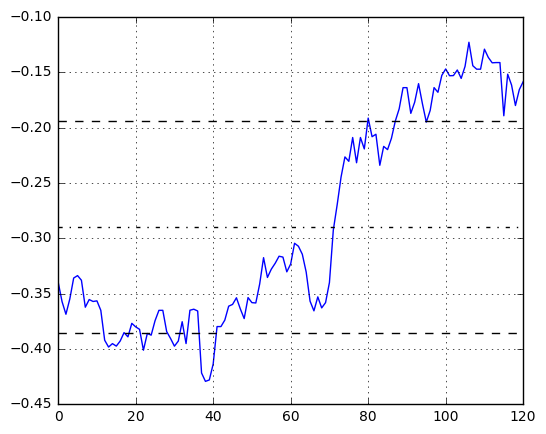
\includegraphics[width=0.9\columnwidth]{graphics/deviation-magnitude.png}
    \caption{
%      Log price difference between a pair of assets $(i, j)$ during a period of $T + 1$ time steps, where $T = 120$.
%      Dashed and dotted line represents mean value, and region between two dashed lines represents $\alpha$ standard deviation range from mean value, here $\alpha = 1$; both are calculated in the first $T$ time steps.
%      During the time step $T + 1$, log price difference goes over $\alpha$ standard deviations above mean value of past period of size $T$.
%      This would mean that two of the assets $i$ and $j$ would be added to the graph of preference flow at the time step $T + 1$.
%      Weight $w_{i,j}$ describes current deviation from mean value.
       Razlika log cijena u paru vrijednosnica $(i,j)$ tijekom perioda od $T + 1$ vremenskih koraka, uz $T = 120$.
       Točka-crta linija predstavlja srednju vrijednost, a područje između dviju crtkanih linija predstavlja $\alpha$ standardnih devijacija udaljenosti od srednje vrijednosti; obje mjere su izračunate nad prvih $T$ vremenskih koraka.
       Tijekom vremenskog koraka $T + 1$, razlika log cijena prelazi preko $\alpha$ standardnih devijacija iznad srednje vrijednosti proteklog perioda duljine $T$.
       To znači da će vrijednosnice $i$ i $j$ biti dodane u graf toka preferencija u vremenskom koraku $T + 1$.
       Težina $w_{i,j}^{(T+1)}$ opisuje devijaciju od srednje vrijednosti.
    }
    \label{fig:devmag}
  \end{figure}
  
  Na taj način moguće je konstruirati graf toka preferencija za bilo koji vremenski korak $t \in \left[T, T + 1, \ldots, D-1\right]$.
  U nekim vremenskim koracima moguće je da dobiveni graf bude prazan, ukoliko nijedan par vrijednosnica $(i,j)$ ne zadovoljava (\ref{eq:thresh}).
  Postavljanjem nižih vrijednosti za $\alpha$ dobivaju se gušći grafovi i manje često se događa da je graf prazan, dok se postavljanjem $\alpha = 0$ uvijek dobivaju potpuni grafovi.
%  Thus it is possible to create a graph of preference flow for each time step $t \in \left[T, T + 1, \ldots, D-1\right]$.
%  At some time steps it is possible that the graph could be empty, if it is the case that no pair $(i,j)$ satisfies (\ref{eq:thresh}).
%  Setting lower values for parameter $\alpha$ yields denser graphs, and setting $\alpha = 0$ always yields complete graphs.
  
  \section{Konstrukcija portfelja}
%  We obtain preference for each asset via the potential method, as described earlier in \ref{sub:potential}.
%  By obtaining the measure of preference for each asset it is possible to pick assets for the portfolio.
%  The most preferred assets should be bought while the least preferred should be short-sold if possible.
  Individualna mjera preferencije za svaku vrijednosnicu dobivena je metodom potencijala, na način kako je ranije opisano u \ref{sub:potential}.
  Vrijednosnice s trenutačno najvećom preferencijom preporučeno je kupiti, dok je one s najmanjom preferencijom preporučeno prodati, odnosno \textit{shortati} ukoliko je to moguće.
  
%  Let $\matr{\phi}^{\left(t\right)} = \begin{bmatrix} \phi_1^{\left(t\right)} & \phi_2^{\left(t\right)} & \ldots & \phi_N^{\left(t\right)} \end{bmatrix}$ denote vector of preferences of assets at time step $t$ and $\phi_i^{\left(t\right)}$ denote the preference for asset $i$ at time step $t$.
%  When picking the assets for the portfolio we take into consideration the consistency measure $\kappa$ as well.
%  Lower values of $\kappa$ suggest that we should diversify our portfolio by including some more assets in the order of preference, while higher values suggest that it is safe to do trading with smaller number of assets.
%  Portfolio diversification might be seen as a strategy for protection from fundamental risks, e.g. risk of asset default.
  Neka je $\matr{\phi}^{\left(t\right)} = \begin{bmatrix} \phi_1^{\left(t\right)} & \phi_2^{\left(t\right)} & \ldots & \phi_N^{\left(t\right)} \end{bmatrix}$ vektor individualnih preferenci vrijednosnica u vremenskom koraku $t$ i $\phi_i^{\left(t\right)}$ individualna preferencija vrijednosnice $i$ u vremenskom koraku $t$.
  Pri odabiru vrijednosnica za portfelj, u obzir se također uzima i mjera konzistentnosti $\kappa$.
  Uključivanje mjere konzistentnosti pri odabiru omogućuje zaštitu od fundamentalnog rizika (propadanja neke dionice) putem diverzifikacije portfelja.
  Interpretacija mjere konzistentnosti je sljedeća: niska mjera konzistentnosti sugerira da procjena u sadašnjem vremenskom koraku nije pouzdana, stoga je bolje diverzificirati portftelj uzimanjem većeg broja vrijednosnica, dok visoka vrijednost mjere konzistentnosti sugerira da je sigurno trgovati s manjim brojem vrijednosnica.
    
%  The bound on the assets which will be taken into portfolio is proportional to the consistency measure $\kappa$.
%  Depending on the nature of assets we may tune the consistency measure $\kappa$ to be more or less inclined to diversification by transforming it to $\kappa^\prime$:
  Granica mjere preferencije za vrijednosnice koje će biti uključene u portfelj je proporcionalna mjeri konzistentnosti $\kappa$.
  Ovisno o prirodi skupa koji je na raspolaganju, mjera konzistentnosti može se preinačiti tako da algoritam bude više ili manje sklon diverzifikaciji portfelja, na sljedeći način:
  \begin{equation}
  \kappa^\prime = a + (1 - a)\kappa^b,
  \end{equation}
  gdje je $a \in [0, 1], b \in \mathbb{R}^+$.
  Za vrijednosti $a = 0$, $b = 1$, $\kappa^\prime$ postaje jednak $\kappa$.
  Parametar $a$ regulira utjecaj mjere konzistentnosti na određivanje portfelja: za $a = 0$, diverzifikacija u potpunosti ovisi o mjeri konzistentnosti $\kappa$, dok za $a = 1$ mjera konzistentnosti ne dolazi do izražaja te se u portfelju zadržava samo vrijednosnica s najvećom individualnom preferencijom.
  S druge strane, parametar $b$ regulira diverzifikaciju portfelja: kada je $0 < b < 1$, algoritam je više privržen diverzifikaciji čak i kada je konzistentnost mala, a kada je $b > 1$, algoritam je više privržen diverzifikaciji čak i kada je mjera konzistencije velika.
  
%  For determining the assets that should be held in the portfolio at time step $t$, we find such assets $i$ for which holds:
  Za odabir vrijednosnica koje će ući u portfelj u vremenskom koraku $t$, pronalaze se sve vrijednosnice $i$ za koje vrijedi:
  \begin{equation}
  \phi_i^{\left(t\right)} \ge \kappa^\prime \cdot \Phi,
  \end{equation}
  gdje je $\Phi = \max_j \left\{ \left| \phi_j \right| \right\}$.
  Isto tako, za prodaju se biraju vrijednosnice $i$, za koje vrijedi:
  \begin{equation}
  \phi_i^{\left(t\right)} \le -\kappa^\prime \cdot \Phi.
  \end{equation}
%  For $a = 0$ diversification completely depends on consistency $\kappa$, while for $a = 1$ only the most preferred asset is held in the portfolio (no diversification).
%  On the other hand, when $0 < b < 1$, algorithm is less inclined to diversification even when consistency is low, and when $b > 1$, algorithm is more inclined to diversification even when consistency is high. 
  
  \chapter{Rezultati}
  Skup podataka nad kojim je algoritam testiran uključuje 203 od 500 dionica koje su bile uključene u S\&P indeks u razdoblju od 1. siječnja 1980. do 31. prosinca. 2003.
  Razdoblje uključuje 6261 dan trgovanja, odnosno vremenskih koraka.
  Ukupno 20503 praova dionica je ispitano metodom statističke arbitraže u svakom vremenskom koraku.
  Simulirani su troškovi trgovanja u iznosu 0.10\% za svako obavljeno trgovanje.
  Sažeti prikaz rezultat dan je u tablici \ref{table:results-1}.
  
  Godišnji Sharpeov omjer $S$ definiran je kao omjer srednjeg godišnjeg povrata $\mu_r$ i srednje godišnje volatilnosti $\sigma_r$.
  Analizirana su zasebno trgovanja koja rezultiraju pozitivnim i negativnim profitom, njihova razlika i omjer.
  Mjera preciznosti definirana je kao omjer broja trgovanja koja rezultiraju pozitivinim profitom u ukupnom broju trgovanja.
  Mjera obrtaja \engl{turnover ratio} opisuje promjenu portfelja između dva vremenska koraka.
  Ova mjera može biti u rasponu od 0 do 2, gdje vrijednost 0 znači da nema promjene, vrijednost 1 odgovara prelasku iz ili u prazan portfelj, a vrijednost 2 znači da su vrijednosnice između dva vremenska koraka potpuno različite.
  Konačno, izračunat je ukupan profit uz uključene troškove trgovanja.
  
%We test the proposed method on a set of 203 stocks that were contiguously included in S&P 500 index from Jan 1st, 1980 thru Dec 31st, 2003, which includes 6261 trading days.
%A total of 20503 pairs of assets were probed for statistical arbitrage at each time step.
%Transaction costs of 0.10% were also included in the analysis.
%The summary of results for various parameters is shown in Table I.
%The annual Sharpe ratio [11] is defined as: S = μ σ r r – the ratio between annual mean returns and volatilities of the considered portfolio.
%For each individual trade we analyze the profit by evaluating the amount of gain, loss and net profit, as well as gain/loss ratio.
%We measure the algorithm accuracy as the ratio of trades resulting in gain to the total number of trades, and we calculate the average turnover ratio as the average percetnage of the portfolio which needs to be rebalanced at each point.
%Finally, we include the transaction costs and recalculate the portfolio gains.
%The highest profits and Sharpe ratios have been achieved when using α = 0.
%These results indicate that the proposed method does indeed yield portfolios which are able to perform mutli–criteria statistical arbitrage on a large set of assets.
%In addition, we report that the method adapts to the inconsistence of preferences by picking variable number of assets into the portfolio.
%This speaks to the resilience of the algorithm to various market conditions, also demonstrated by the obtained portfolio performance.
%Another interesting finding is the fact that the average gain is much higher than the average loss, meaning that the algorithm errors cost less than the gains obtained when the algorithm is correct.
%The method is shown to produce rational turnover ratios, and the fact that the obtained Sharpe ratios remain high despite transaction costs additionally affirms the validity of the approach
%These findings suggest that the proposed method produces consistent returns and may be feasible in a live market setting.
  
  \begin{sidewaystable}[p]
  \centering
  \captionof{table}{Rezultati testiranja nad S\&P 203 skupu, uz $T = 60, \beta=0$.}
  \label{table:results-1}
  \begin{tabularx}{\hsize}{Xrrrrrrr}
    \toprule
    Parametar: & & & & & & & \\
    \quad a & \multicolumn{3}{c}{0.0} & \multicolumn{3}{c}{0.5} & \multicolumn{1}{c}{1.0} \\ \cmidrule(lr){2-4} \cmidrule(lr){5-7} \cmidrule(lr){8-8}
    \quad b & \multicolumn{1}{c}{0.5} & \multicolumn{1}{c}{1.0} & \multicolumn{1}{c}{2.0} & \multicolumn{1}{c}{0.5} & \multicolumn{1}{c}{1.0} & \multicolumn{1}{c}{2.0} & \multicolumn{1}{c}{/} \\ \midrule
    Prosječni povrat (godišnji) & 0.95339 & 0.88967 & 0.84463 & 0.98336 & 0.95663 & 0.89704 & 1.00223 \\
    Volatilnost (godišnja) & 0.77042 & 0.76595 & 0.74077 & 0.77905 & 0.77054 & 0.76660 & 0.78363 \\
    Sharpeov omjer (godišnji) & 1.23750 & 1.16152 & 1.14020 & 1.26225 & 1.24150 & 1.17015 & 1.27896 \\ \midrule
    Profit: &  &  &  &  &  &  &  \\
    \quad samo pozitivan & 89.27624 & 88.89440 & 88.32548 & 89.58775 & 89.29840 & 89.04414 & 89.55020 \\
    \quad samo negativan & -58.37779 & -59.03715 & -58.41396 & -58.24852 & -58.32385 & -59.02220 & -58.05316 \\
    \quad ukupan & 30.89846 & 29.85725 & 29.91152 & 31.33923 & 30.97456 & 30.02195 & 31.49704 \\
    \quad omjer pozitivnog i negativnog & 1.52928 & 1.50574 & 1.51206 & 1.53803 & 1.53108 & 1.50866 & 1.54256 \\ \midrule
    Prosječna točnost & 0.36485 & 0.39276 & 0.43413 & 0.34902 & 0.36458 & 0.39145 & 0.33241 \\
    Prosječni koeficijent obrtaja & 0.59976 & 0.64224 & 0.73597 & 0.57585 & 0.59947 & 0.64089 & 0.55112 \\ \midrule
    Stvarni profit, uz troškove trgovanja od 0.10\% & 23.46019 & 21.89215 & 20.78402 & 24.19757 & 23.53996 & 22.07361 & 24.66204 \\
    \bottomrule
  \end{tabularx}
\end{sidewaystable}


  \chapter{Zaključak}
  Algorithm works on pairs of assets, looking for those deviations which are uncommon, so generally it is expected to perform better where there is larger number of assets as more deviations will be discovered.
  It adapts to the inconsistence of preferences by picking variable number of assets into the portfolio.
  
\bibliography{literatura}
\bibliographystyle{unsrtnat}

\appendix
\chapter{Efikasno računanje momenata s pomičnim prozorom}
Pri izračunavanju momenata (srednja vrijednost, varijanca) vremenskih nizova 

\begin{sazetak}
Sažetak na hrvatskom jeziku.

\kljucnerijeci{Ključne riječi, odvojene zarezima.}
\end{sazetak}

% w: Navedite naslov na engleskom jeziku.
\engtitle{Complex network based time series analysis}
\begin{abstract}
Abstract.

\keywords{Keywords.}
\end{abstract}

\end{document}
